%%%%%%%%%%%%%%%% Relojes Bloom.
\begin{frame}[fragile]{Relojes Bloom:}{Filtro Bloom. Mejoras.}
  \justifying
  ¿Qué podemos hacer? ...\newline
  Podemos usar una variante de \textit{bloom-filtros} con conteo
  de entradas, como se muestra en el siguiente ejemplo:
    \begin{figure}
    \centering
    \begin{subfigure}[b]{0.5\textwidth}
      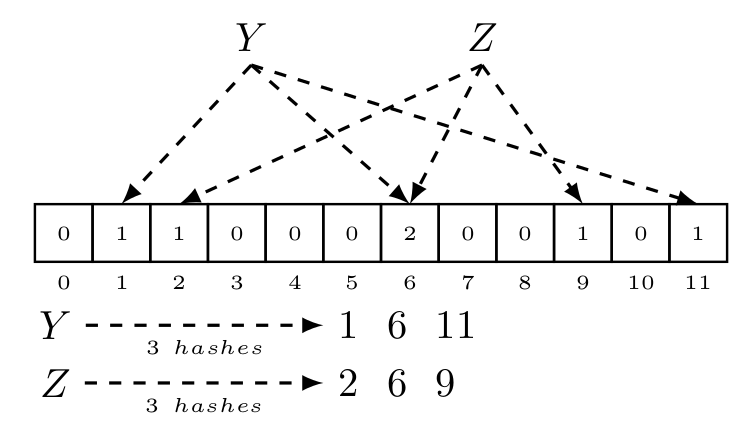
\includegraphics[width=\textwidth]{./Imagenes/CountingBloomClock}
      \caption{Filtro de Bloom tipo contador.}
      \label{fig:Ejemplo de un CountingBloomClock.}
    \end{subfigure}
  \end{figure}
\end{frame}
